\documentclass[10pt,twoside,openright]{report}
\usepackage{graphicx} 
\usepackage{amsmath}
\usepackage[hyphens]{url}
\usepackage[driverfallback=dvips,unicode=true,bookmarks=false,
    bookmarksopen=false,pdfpagelabels=false,pdfstartview={FitH},pdfpagelayout=TwoPageRight,
    pdfborder={0 0 0},pdfdisplaydoctitle=true,bookmarksnumbered=false,
    backref=false,breaklinks=true,colorlinks=true,citecolor=black,
    filecolor=black,linkcolor=black,urlcolor=black,hypertexnames=false]{hyperref}
\hypersetup{pdftitle={Empowering Under-Served Voices in Spoken Language Interaction},
    pdfauthor={The UnMute project team and collaborators},pdfsubject={},pdfcreator={},pdfproducer={},pdfkeywords={}}
\usepackage{amssymb}
\usepackage{caption}
\usepackage{subcaption}
\usepackage{xcolor}
\usepackage{bm}
\usepackage{titling}
\usepackage{algorithm2e}
\usepackage{overpic}
\usepackage{enumitem}
\urlstyle{same}

\usepackage{caption}
\captionsetup{labelformat=empty,justification=centering,font=small,labelfont=small}

\usepackage[papersize={154mm,216mm},layouthoffset=3mm,layoutvoffset=3mm,layout=a5paper,
    top=2.5cm,bottom=1.8cm,inner=2.4cm,outer=1.8cm,headsep=1.8cm]{geometry}
\usepackage{sectsty}
\allsectionsfont{\sffamily}
\usepackage{microtype}
\usepackage{pdfpages}
\usepackage{tikz}

\usepackage{zref-savepos}
\setcounter{secnumdepth}{0}
\newcommand\headingbackground[1]{\zsavepos{chapterPos\the\value{chapter}}
\AddToShipoutPicture*{
\ifthenelse{\equal{#1}{}}{
\chapterBox{\dimexpr\paperheight-\zposy{chapterPos\the\value{chapter}}sp-2em\relax}}{
\mainChapterBox{\dimexpr\paperheight-\zposy{chapterPos\the\value{chapter}}sp-2em\relax}}
}}
\newcommand\tocchapter[2][]{\chapter*{#2}%
\addcontentsline{toc}{chapter}{#2}%
\refstepcounter{chapter}\headingbackground{#1}}

\usepackage{ragged2e}
\usepackage[parfill]{parskip}
\frenchspacing
\usepackage{setspace}
\spacing{1.2}

\usepackage{fontspec}

\usepackage{titlesec}
\usepackage{xcolor}
\usepackage{eso-pic}
\usepackage{geometry}
\usepackage{zref-savepos}
\definecolor{unmutedarkcolour}{RGB}{94,24,92}
\definecolor{unmutelightcolour}{RGB}{121,51,120}
\setsansfont{Agrandir-TextBold.otf}
\setmainfont{TeXGyrePagellaX}

\newcommand\chapterBox[1]{%
  \put(0,0){%
    \parbox[b][\paperheight]{\paperwidth}{%
      \color{unmutelightcolour}\rule{\paperwidth}{#1} %
      \vfill
    }
}}

\newcommand\mainChapterBox[1]{%
  \put(0,0){%
    \parbox[b][\paperheight]{\paperwidth}{%
      \color{unmutedarkcolour}\rule{\paperwidth}{#1} %
      \begin{tikzpicture}[overlay]%
        \node (image) at (1.2,7.1) {
\includegraphics[scale=0.25]{media/waves.pdf}};
        \node (image) at (12.2,7.3) {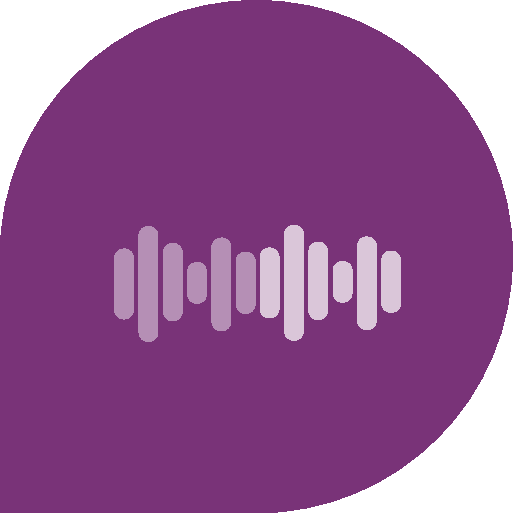
\includegraphics[scale=0.9]{media/bubble_decorated.pdf}};
      \end{tikzpicture}
      \vfill
    }
}}

\titleformat{\chapter}[display]
            {\color{white}\huge\sffamily\raggedright}
            {}
            {0cm}
            {\thispagestyle{empty}\begin{spacing}{0.8}}
            [\end{spacing}] %
\titlespacing*{\chapter}{0pt}{40pt}{70pt}

\newcommand\notes[1]{\textcolor{red}{#1}}
\newcommand\figures[1]{\textcolor{blue}{#1}}

\title{Empowering Under-Served Voices in Spoken Language Interaction}
\author{UnMute Report No. 1}
\date{January 2024}



\newcommand{\currentpart}{}
\newcommand{\unmutepart}[1]{\clearpage%
    \renewcommand{\currentpart}{#1}}

\makeatletter
\newcommand*{\shifttext}[2]{%
  \settowidth{\@tempdima}{#2}%
  \makebox[\@tempdima]{\hspace*{#1}#2}%
}
\makeatother

\makeatletter
\def\ps@unmute{%
\def\pagethreshold{10}%
\def\@oddhead{\AddToShipoutPictureBG{\AtPageUpperLeft{\textcolor{unmutelightcolour}{\rule[-1.3cm]{\paperwidth}{1pt}}}}%
    \reset@font\hfil\shifttext{2.7cm}{\textcolor{unmutelightcolour}{\sffamily\textbf{\currentpart%
\ifnum\value{page}<\pagethreshold%
    \hspace{3.1em}%
    \else%
    \hspace{2.7em}%
   \fi%
\thepage}}}}%
  \def\@evenhead{\AddToShipoutPictureBG{\AtPageUpperLeft{\textcolor{unmutelightcolour}{\rule[-1.3cm]{\paperwidth}{1pt}}}}%
    \reset@font\shifttext{-2.7cm}{\textcolor{unmutelightcolour}{\sffamily\textbf{\thepage%
\ifnum\value{page}<\pagethreshold%
    \hspace{3.1em}%
    \else%
    \hspace{2.7em}%
   \fi%
    \currentpart}}}\hfil}%
  \let\@oddfoot\@empty%
  \let\@evenfoot\@empty%
}
\makeatother

\makeatletter\newenvironment{unmutehighlight}{
	\setlength\fboxrule{3.0pt} %
	\setlength\fboxsep{8.0pt} %
	\par\begin{centering}\color{white}\vspace{2em}
	\begin{lrbox}{\@tempboxa}
	\begin{minipage}{\dimexpr\columnwidth-2\fboxrule-2\fboxsep}}{
	\end{minipage}
	\end{lrbox}
	\fcolorbox{white}{unmutelightcolour}{\usebox{\@tempboxa}}
	\end{centering}\par
}\makeatother

\begin{document}
\RaggedRight


\thispagestyle{empty}
\unmutepart{Welcome}
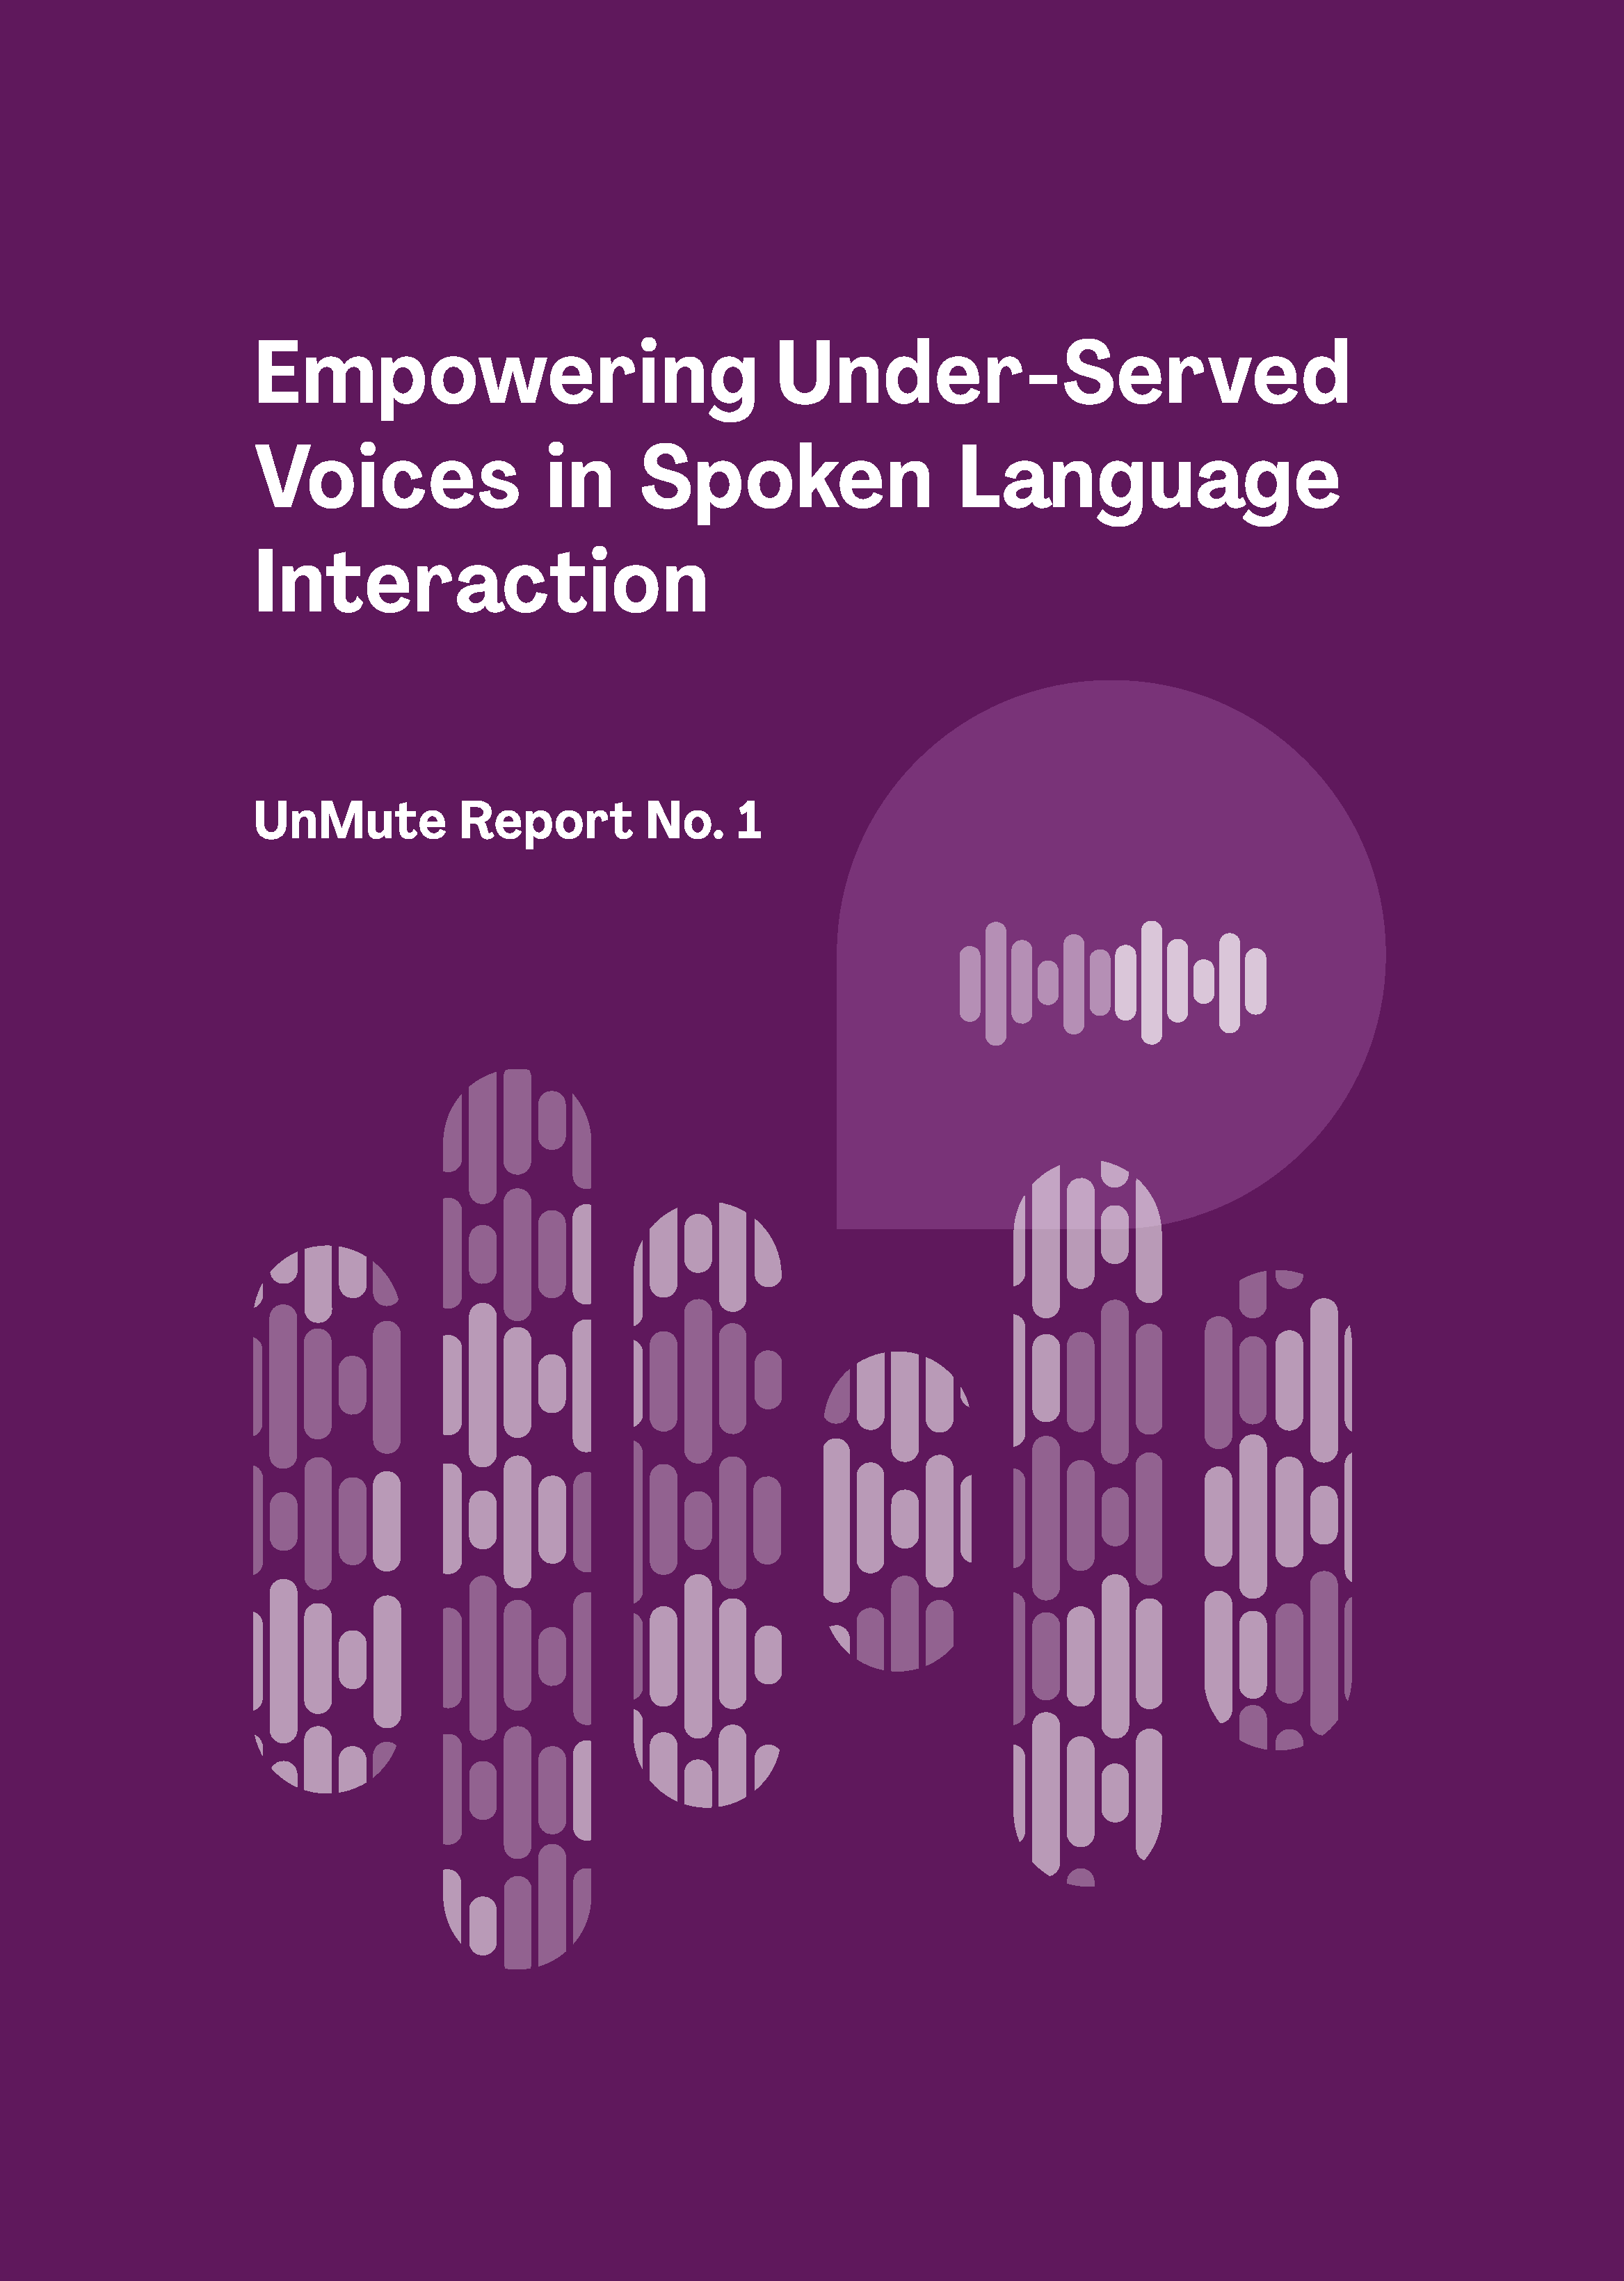
\includepdf[pages={1},offset=0 0mm,height=218mm]{media/cover-front}

\clearpage

\thispagestyle{empty}
\begin{centering}
\textbf{Acknowledgements}

We would like to thank all of the participants who contributed to the co-design activities described in this report.

The work reported here was funded by EPSRC grant EP/T024976/1 and RAI grant IA012.\\
\end{centering}

\vfill

{\footnotesize This report was co-authored by a multidisciplinary team from the UK and India:

Peter Bell (Centre for Speech Technology Research, University of Edinburgh)\\
Matt Jones (Future Interaction Technology Lab, Swansea University)\\
Ond{\v{r}}ej Klejch (Centre for Speech Technology Research, University of Edinburgh)\\
Nina Markl (Institute for Analytics and Data Science, University of Essex)\\
Jennifer Pearson (Future Interaction Technology  Lab, Swansea University)\\
Dani Raju (Studio Hasi, Mumbai)\\
Thomas Reitmaier (Future Interaction Technology  Lab, Swansea University)\\
Simon Robinson (Future Interaction Technology  Lab, Swansea University)\\
\mbox{Electra Wallington (Centre for Speech Technology Research, University of Edinburgh)}\\ %
}


\tocchapter[Welcome]{Empowering Under-Served Voices in Spoken Language Interaction}
\pagestyle{unmute}
\section{Executive summary}
Speech is one of the richest forms of human communication.
But speech-based interactive systems are currently available for only a small fraction of the world's languages.
Consequently, hundreds of millions of people are being excluded globally.

For the past three years we have worked with so-called ``low-resource'' language communities as part of a research project---UnMute---to explore responsible and inclusive techniques for developing speech recognition with low data requirements.
In this report we explore the motivations, challenges and benefits of working with under-served communities such as these to develop automatic speech recognition tools and associated interactive services.

We argue for inclusive technology design and data-compilation methods, present our approach, and detail case studies showing examples of its potential.
We provide a toolkit for developing speech technologies for language varieties for which there are---for complex historical and sometimes socio-cultural reasons---very little written, computer-readable text data which would traditionally be required for technology development.
All of the contributions presented in this report are open-source, and we invite you to get involved in shaping and improving the approach we describe.

\begin{unmutehighlight}
\section*{Key themes}
\begin{itemize}[itemsep=1em]
\item It is valuable---indeed essential---to work with speakers of low-resource languages when developing new speech technologies.
\item Inclusive approaches to design and data-collection bring benefits to both developers and end-users.
\item Insights from low-resource language speakers can inform design for the rest of the world.
\end{itemize}
\vspace{0.5em}
\end{unmutehighlight}


\unmutepart{Important Concepts}
\tocchapter{Important Concepts}
The team behind this report is an interdisciplinary group of Human-Computer Interaction (HCI), Artificial Intelligence (AI) and Linguistics researchers designing a set of resources to be used by both language communities and other interdisciplinary teams.
Before diving into the rest of this report, we provide some brief definitions for key terms and concepts.
This is especially important as some of these terms may be prevalent, or of common use, within one field but not another, or else else have slightly different meanings or connotations across different disciplines (for instance between the fields of AI and Computer Science, HCI, and Sociolinguistics).

\textbf{Speech and Language Technologies:}
We use this term to reference the subset of the AI discipline which focuses on facilitating natural interaction between people and computers via spoken or written language (with the computer/device being able to produce, modify, and/or respond), or else enabling the computational analysis of text and speech.

\textbf{Automatic Speech Recognition (ASR):} An example of a speech and language technology.
The goal of an ASR system is to recognise incoming speech and convert it to a textual representation.
This textual representation could be outputted and shown to an end-user directly if the system's use-case necessitates this, for example if the system is being used to transcribe audio conversations to be looked back upon.
An ASR model could also be embedded into a larger system, whereby its outputted ``textual representation'' is passed onto another component, such as a search engine, thus only being used internally and unseen by the end user.

\textbf{Low-resource/under-resourced [languages]:} In the context of speech and language technology development, languages are sometimes described as being ``low-resource''.
These varieties are characterised by a comparative lack of the kinds of data typically required to develop speech and language technologies (speech and text data-sets).
Not all ``low-resource'' languages are spoken by small numbers of speakers.
However, many, if not most, could be considered (historically) minoritised, for example in colonial contexts.
Because the apparent ``lack'' of resources often goes hand in hand with wider economic inequality and injustice, the term has been critiqued in recent years.
Alternative framings such as ``under-resourced'' or ``under-served'' communities and languages may better reflect these complex political and historical legacies. 


\unmutepart{The UnMute Approach}
\tocchapter{Introducing our Approach}
\section{Why should we want to build speech and\texorpdfstring{\\}{ }language technologies for under-served\texorpdfstring{\\}{ }languages and communities?}
\label{sec:intro}
Speech and language technologies---facilitated by recent advances in hardware and cloud computing---are increasingly being integrated into products and services used daily by millions of people across the globe.
For many people, such technologies have simplified a wide range of tasks (e.g., voice assistants to operate smart homes, computers and mobile phones).
Whether these tools are merely convenient or an important accessibility tool depends on users' individual circumstances, but either way, they have become embedded in many people's professional and private lives. 

However, there remain huge disparities regarding the languages---and therefore communities---for which these services are available.
While many large commercial providers of language technologies (such as Google, Apple and Amazon) support a growing number of language varieties, availability still tends to be skewed towards ``high-resource'' languages and those primarily spoken in territories which are of high commercial interest to these companies. 

Speech and language technologies have a lot to offer to communities who speak languages that are currently unsupported.
Devices equipped with speech interfaces do not require users to be able to read or write in a specific script or interact with a keyboard or touchscreen.
Since many language varieties across the world are not associated with a particular native script, and writing practises vary widely depending on the socio-cultural context, these speech interfaces are uniquely accessible to a large proportion of potential users. 

Consider the increased ease of disseminating information to remote communities if such information could be queried by voice.
Increasing digital participation of communities who currently lack access can also support efforts to document, revive and transmit endangered and minoritised language varieties and their associated cultural practises.
In short, AI and speech and language technologies---if developed responsibly and inclusively---can amplify the voices of those who are currently unheard.


\section{Why has this traditionally been difficult~\texorpdfstring{\raisebox{3pt}{\rule{8pt}{1.5pt}}}{--} and is this still the case?}
Traditionally, to train a high-quality Automatic Speech Recognition (ASR) system for a new language, use-case or domain would require a large data-set of recorded speech carefully matched with precise verbatim transcriptions (known as ``labelled'' data).\footnote{Note that we use ASR as an example use-case throughout this report but that similar applies to development of systems across most speech/language technology disciplines (e.g., speech synthesis, machine translation and so on).}
With sufficient examples of speech and text, the system can ``learn'' a mapping between these two modalities.
Once learnt, this mapping---or ``model''---can be used with new, previously unseen audio.

However, large quantities of parallel speech and transcription data are simply not available in many contexts.
While compiling and storing speech samples themselves has become easier in recent years, sourcing high-quality transcriptions is labour-intensive and often involves complex negotiations around language representations and competing transcription conventions.
This of course assumes that the language has a written form at all, which is not always the case.
Recent years have therefore seen a considerable push towards developing alternative ``low-resource'' ASR training methods.

The approach which has perhaps experienced the largest boom in dedicated research utilises what is known as ``self-supervised learning'' and splits the training of such systems into two phases.
First, extremely large amounts of \textit{untranscribed} speech are used to train a base language model.
Only after this point is target domain or language data utilised: a second phase takes these somewhat language-agnostic base models and transforms them---via ``fine-tuning''---into ones that \textit{are} language- or domain-specific.

Because this method lessens the reliance on large language-specific labelled training data-sets; and, of course, because unlabelled audio data for a new language is so much easier to obtain, advancements in these self-supervised models or pipelines have facilitated the building of systems for languages which we could not have previously developed models for. 

It is important to highlight that the unlabelled audio data requirements here are far greater than what is required for other approaches: tens of thousands of hours are needed, across as many different languages or domains as possible.
This of course also entails huge computing and storage requirements.
Because of this, these approaches are increasingly the exclusive provenance of large technology organisations that are able to afford the cost of training new models.\footnote{Consider, for example, Facebook AI's `wav2vec 2.0' ASR framework, in theory supporting more than 7,000 languages spoken worldwide, which required 53,000 hours of unlabelled speech data to build.
Other approaches require even more data~-- for example, OpenAI's `Whisper,' which was trained using 680,000 hours of audio.}


\vspace{-1em}
\begin{unmutehighlight}
\section*{The importance of testing}
An equally important (though sometimes overlooked) aspect of the ASR development pipeline is testing of a language model's quality.
We must be able to compare the suitability of different design choices for the specific context---different model architectures, data pre-processing techniques, decoding algorithms and so on---and adjust parameters in response.

\vspace{1em}

In ASR, the typical measure is Word Error Rate (WER), which is defined as the number of errors in the system's output divided by the number of words in a known correct output.
The intuitive nature of WER coupled with its computational simplicity makes it the most popular measure of performance in this area.
Like in other areas of AI development, metric-based indicators of performance have become a key measure of success and merit in discussions of speech and language technology in academic research, advertising and the media.

\vspace{1em}

This focus on easy-to-compute, ``objective'' metrics %
means relatively large and representative transcribed data-sets are still required to evaluate performance.
More importantly, it also means that while some research attention may have shifted towards under-resourced languages, their speakers' experiences with the technology are not often placed at the forefront.
Understanding how and why communities use language technologies and how they judge their performance is particularly important when developing with and for multilingual and/or marginalised communities.
Many of the standard development paradigms assume that users are monolingual and experienced with digital technologies, for example.
This assumption is often in direct conflict with real lived experiences.
\end{unmutehighlight}


\section{What is missing from current ``low-resource''\texorpdfstring{\\}{ }ASR development pipelines?}
So far we have considered why we should want to be able to build speech and language technologies for under-resourced language communities; we have discussed why building ASR systems for such contexts has traditionally been difficult; and, finally, we have looked at how recent work in the ASR research community has been responding to these ``low-resource'' gaps. 

The question that remains is, in order to fulfil this ideal scenario where we could work with \textit{any} new language community and be confident we had the means to provide some kind of speech or language system, is there still work to to be done? 

We believe the answer to this question is \textbf{yes}.
More importantly, we believe that even if the research areas that are currently directly responding to low-resource language development challenges continue to be pursued---and those methodologies affiliated with these areas continued to be refined---this would still not be sufficient to meet this goal.
Why is this the case?


\subsection{We need alternative ASR training frameworks\ldots} 
There is no doubt that the breakthroughs regarding self-supervised models have enabled ASR researchers to build systems for languages and contexts that simply could not have been approached in the past.
But, as we mentioned above, the training and hosting of these systems is limited to only those few organisations (mostly large corporations) which have sufficient resources (in terms of data, computation infrastructure, skilled labour and money).
This reliance on large technology companies and, to a lesser extent, academic institutions, mostly situated in the Global North, is a cause for concern for many.
It arguably replicates and extends long-standing power inequities between the Global North and Global South, and raises important questions regarding data sovereignty of language communities. 

The research community must also remember that these approaches have not yet provided anywhere near an exhaustive coverage of the world's languages.
Nor necessarily can they.
Self-supervised models and similar approaches rely on the learning of general language features which are then transferable and generalisable across languages and domains.
However, even if the data sources from which these features are learnt are extensive, the distribution of this data will still embed biases regarding the language typologies, styles and speakers that are represented.
Large multilingual self-supervised models have been shown to work far less well for languages which are typologically very different from the ``well-resourced'' languages that comprise the bulk of available data-sets. 


\subsection{\ldots that complement, and can be embedded within,\texorpdfstring{\\}{ }self-driven, community-focused ASR development}
If ASR development continues to be constrained solely (or primarily) ``to the lab'' such that we bypass the communities for whom we are supposedly developing these systems, we risk misjudging or misunderstanding what exactly it is we should be modelling to begin with or, at the very least, missing out on getting the whole picture. 
That is, we risk embedding biases into our systems; we risk making assumptions or being naive with regard to the extent of the target language's features or community's needs; we risk, generally, making our development pipelines slightly circular, working towards a target that has been, to some extent, self-imposed.

That is, many of the languages of the world are very often represented online only in particularly constrained, formal contexts: official documentation, for instance, or else government websites, or educational resources.
And what is dangerous about this is that the linguistic features common in conversational speech---blended multi-language use (``code-switching'') and the prominence of multilingualism being one very prevalent example %
across many under-represented communities---can be heavily diluted, or even completely undetectable, within these domains.
This is not to mention that the enforced or prescriptive ``standards'' constraining speech and text in these regulated contexts may carry or evoke specifically negative attitudes, connotations or responses in speakers themselves if heard in day-to-day life.

We believe, however, that these risks can to a large extent be circumvented.
Specifically, we posit that this circumventing starts by accepting just how nuanced the challenge of developing speech and language technologies for diverse communities can be \textit{and} that we can actually enrich our research and development pipelines by engaging with and learning from the communities for whom we are meant to be working.

Consider the problem of unrepresentative online data leading to potential evaluation circularities.
What if we knew precisely how best to work \textit{with} community members to create test data-sets or materials, or else to carry out quantitative or qualitative community-led evaluation procedures supplementary to standard in-the-lab evaluation metrics?
Consider also the very real chance of researchers---whether intentionally or unintentionally---imposing prescriptive standards or making naive assumptions when designing systems: choosing how our system output should be presented, for instance; or even deciding on system use-cases to begin with.
It seems sensible, given this, to ensure our approaches have, embedded within them from the very start, constant communication between teams ``in the lab'' and community members with whom we are designing.

In short, research efforts are currently centred on the refining of methods of large-scale data mining; the hosting of language models; and, means of learning everything we need to know ``from the data''.
We believe it is equally important to integrate the topics of community-engagement; how to integrate community co-design and feedback into existing work and methodologies; and, generally, how best to establish more bi-directional, ground-up development pipelines which put communities at the fore, and therefore ground research and development in the real world.


\section{Our approach: a report overview}
The remainder of this report is split into two key sections. 

\subsection{1: Guidelines for establishing a community-led,\texorpdfstring{\\}{ }spoken language technology development project} 
Regardless of the specific technology being built or language community being partnered with, our approach advocates for consistent ``ground-up'' community-centred development.
Therefore, in this first section, we offer a series of flexible, generalisable %
guidelines and principles that can aid the initial establishment of such a community-led project, and improve its likelihood of success.
\subsection{2: A pipeline for community-centred speech\texorpdfstring{\\}{ }technology development with un-written languages}
Our second offering is more specific.
We present a case study of a \textit{complete} pipeline which enables the building of a spoken-content retrieval system system from seed (that is, neither assuming nor requiring existing language resources) and, importantly, is compatible with solely oral (i.e., un-written) low-resource languages.

All of the contributions described in this report are open-source, and available for others to build upon and extend.
Further detail, instructions and guidance can be found on our website: \underline{\href{https://unmute.tech/}{www.unmute.tech}}.


\unmutepart{Inclusive spoken language technology development}
\tocchapter[Section 1]{Guidelines for Inclusive Spoken Language Technology Development}
\section{Introduction}
In this section we provide guidelines that can be followed when initially establishing an inter-disciplinary, community-centred language technology project.
We propose key questions that must be considered when assembling a team; we provide frameworks and case-study examples which can be referenced when initially exploring and engaging with a language community; and, we offer a list of questions and features that should be understood about a language community before engaging in any further development.
We also provide blueprints and general tips that can be referred to when hosting community workshops and participant trials (which we would recommend conducting \textit{throughout} the entire development process: before any system building; for evaluation purposes, etc).

Some of the questions and topics in this section may seem rudimentary to those who have been working in this area for some time.
However, given the importance in our view of fundamentally changing the way that ``low-resource'' speech technologies are developed, we believe it is important to provide a detailed overview as an introductory guide to anyone interested in speech and language technology.
Given how integral we believe community understanding and engagement should be to spoken language technology development, we very strongly recommend that this section is consulted prior to the undertaking of subsequent system development stages. 


\tocchapter{Getting Started}
\section{Identifying a community liaison}
To kick off such a development project, we would recommend first identifying a community liaison (also sometimes known as a ``human access point'').
This person should be someone who is trusted in the community and speaks the community's language, but simultaneously can communicate with the research team and maintain regular contact over an extended period.
It is beneficial if the liaison is familiar with how to formulate research tasks and trials, such that they can help situate design activities and facilitate uptake during workshops and deployments.
The community liaison should be seen as the first point of contact and a ``critical friend'' who can provide any immediate thoughts or feedback, or tips on how to proceed given knowledge of the community and their practices. 


\section{Assessing existing technological, ethnographic\texorpdfstring{\\}{ }and linguistic accounts}

Before undertaking any practical or in-person work, spend time understanding existing ethnographic accounts, and linguistic or computational research surrounding the language community (if such documentation exists).
Particular topics of value include:
\begin{itemize}
    \item What is the geographic spread of the community?
    Is it near other communities or settlements?
    Does the community keep to itself or interact with these other communities?  
    \item Does the community speak one language primarily/exclusively, or is multilingualism or code-switching common?
    If the latter, are different languages constrained to different scenarios or contexts?
    Do community members tend to learn the languages of nearby communities as second languages? 
    \item What is the social and political history of the community?
    Is this reflected in language or cultural practices in any way?
    \item Does the community's (primary) language have its own script?
    Is it commonly written if so?
    If not, is transliteration used?
    \item To what extent does the community's (primary) language have an online or digital presence?
    Is this constrained to particular domains? 
    \item What are the technical/digital literacy levels within the community?
    What type of technologies are used in the community on a day-to-day basis, and what types of technologies would be unfamiliar? 
\end{itemize} 

Any information identified here can help to guide initial exploratory, face-to-face community-based research, questions, or workshops. 

\begin{unmutehighlight}
\section*{Why observation matters}
Before undertaking a project in collaboration with a Banjara community, we \textit{did} find a small number of linguistic resources such as word-lists and multi-lingual dictionaries.
Ethnographic accounts from previous researchers discussed transliteration,
\end{unmutehighlight}

\vspace{-3.5em}
\begin{unmutehighlight}
stating that this was a fairly commonly undertaken practice.
However, early into our visits, we quickly found that practices vastly diverged from these academic accounts: there was little evidence of transliteration.
\vspace{0.1em}
\end{unmutehighlight}
\vspace{-0.1em}


\section{Learning, participating and contextualising}
Even more useful than remote research is experiencing, observing and learning from community members first-hand.
If possible, we strongly recommend that as part of the initial exploratory/formative phase, at least some of the technology team visit the community and partake, document and report back on activities and everyday practices.

Such an exploratory research visit need not be extensively structured: we would recommend accompanying one's hosts and observing and engaging in as much of daily life as possible, discussing and asking for demonstrations opportunistically.
Findings can be communicated to remote research team members via log-books, as well as photos or videos.

During this observing and engaging, the sorts of questions that we listed in the previous section should be returned to.
Namely, how is language being used in the community; and, importantly, do the observed real life practices surrounding language use match up with those documented in existing sources?
Explicit discussion prompts (with groups or with separate community members) could be beneficial here to delve deeper into topics such as code-switching and multilingualism: do different languages carry different emotional weight or cultural significance, for instance? 

Some further features that are worth documenting and reporting back on during this phase include: 
\begin{itemize}
    \item What are the general practices surrounding mobile phone or other device ownership, use, and sharing? Is mobile phone signal available? What is the cost of mobile data? 
    \item What are the audio conditions like in the community?
    Are there any spots where one could record in quiet conditions?
    Do daily practices mean that extended periods of time without interruption are unlikely?
\end{itemize}

Throughout this phase, it is particularly important to engage with different groups within the community---different age groups; different social groups; different gender groups---and to understand how answers to the above posed questions may differ depending on demographic.
Any variation here (and there will most likely be variation) may have an important bearing on how later collaborative design tasks or data collection methods are designed.

\vspace{-0.8em}
\begin{unmutehighlight}
\section*{Styles of engagement}
There will likely be generational differences in terms of digital literacy and confidence when using technological devices.
We have been mindful of this by, for example, asking younger community members to kickstart data-collection processes, and then helping to explain these processes to older community members. 
There may also be differences between men and women regarding narration/speech styles, amplitudes, or confidence when interacting with data collection probes or else spoken technology systems themselves.
Finally, it is important to consider different group roles and schedules within the community when conducting workshops or tasks.
\end{unmutehighlight}

Such an exploratory visit is a good opportunity to begin to get a sense of particular use-cases or domains that may be of specific relevance to the language community~-- after all, we want the system we build to actually be useful and tailored to the people with whom we are working.
Prompts that can be considered here include:

\begin{itemize}
    \item What jobs (if any) do people spend most of their day doing? What do people do in their free time or to relax?
    \item What place do farming, cooking, shopping, building and other key tasks have in the community?
    \item How is important information (for example, medical advice) disseminated to and within the community? How is digital and other media exchanged or shared?
    \item What are the communication channels like within the community, or between neighbouring communities (or between families/friends in different regions)? 
\end{itemize}

Finally, it is worth emphasising that while you may find yourself asking lots of questions, partnership and reciprocity are key.
Watch and understand, but share willingly, and be eager to learn.


\makeatletter
\@openrightfalse
\makeatother

\tocchapter{Contextualising Ideas and Technologies}

\makeatletter
\@openrighttrue
\makeatother

\section{Formulating an idea: consolidation and\texorpdfstring{\\}{ }preparatory workshops}
Having undertaken this initial exploratory phase, a research team can then begin to formulate more specific plans regarding system aims, designs, and means.
The following questions are useful to consider as part of this formulation: 
\begin{itemize}
    \item What potential use-cases have been identified?
    How could a spoken language system benefit this community?
    Are there specific domains for which such a system would be best suited?
    \item What should be the aim of the spoken language technology system we are hoping to  develop?
    \item How should the task be formulated from a mathematical/ computational perspective? 
    \item What types of data are accessible?
    Is this sufficient to facilitate system building even with low-data approaches?
    \item How can the system be tested---quantitatively and qualitatively---to allow for iterative improvement?
\end{itemize}

After initial idea brainstorming, we recommend returning to the community (in person, or else remotely whilst maintaining strong contact with the community liaison): this time, to host more structured and focused workshops or discussions centred around the appropriateness of these ideas, and the validity of their implementation.
At this point, the following activities may be of benefit: 
\begin{itemize}
    \item Discussing possible domains and use-cases and obtaining feedback.
    \item Explaining the system to be designed as well as the development process (at a high level) to community members.
    This could incorporate examples of the design's workings, and asking for feedback/ensuring understanding at each stage. 
    \item Trialling and testing any processes, hardware or software that may be used during development (e.g., data-collection).
    In light of feedback, such processes, hardware or software tools may then need to be adapted opportunistically.
    \item Training community members to use any processes, hardware or software that may be required (e.g., data-collection methods; evaluation tools). 
\end{itemize}

Such activities provide a great opportunity to refine methods or tools, and overall increase the likelihood of development success from a procedural point of view.
In addition, these activities are important to provide more detail and give a better sense of possible outcomes to community members, but also to ground the development process as something that truly involves the community, and can indeed be changed or revised as needed.


\section{Illustrating speech and language technologies}
In order for responsible, inclusive spoken language technology development to truly live up to its description, it is important that community members understand why they are doing what they are doing throughout the development of a new speech system.
If communities understand exactly what it is that is being constructed; and, at a high level, how it might work, and how we are planning to go about building it, then participants are likely to be more engaged, more enthusiastic, and generally more involved.

\begin{unmutehighlight}
\section*{The value of metaphors}
It can be challenging to know how to begin explaining a highly-technical design to someone unfamiliar with many of the processes involved.
Metaphors can be useful here, because they enable people to relate new, often abstract information to existing things that they \textit{do} know about.

\vspace{1em}

For example, we have used the metaphor of a child who is slowly learning to speak as an analogy for how speech and language technologies ``learn'' a language from repeated exposure to particular utterances, explaining how, with time (i.e., more data), such a system could identify and match similar phrases.
This metaphor is also useful when explaining that speech and language technologies can often make mistakes that seem childish or obvious (to an experienced speaker) in nature.
\vspace{0.1em}
\end{unmutehighlight}


\tocchapter{Responsibility and Integrity}
\section{Planning for inclusion}
As the past few sections demonstrate, there will be many points throughout the co-development of an inclusive spoken language system where community trials, workshops, or general structured engagement will be called for.
For example: 

\begin{itemize}
    \item Exploratory discussions prior to any development
    \item Data collection or checking/quality assurance tasks 
    \item Transcription tasks (of already collected data)
    \item Evaluation tasks during system building or adaptation
    \item Feedback, evaluation and co-design workshops
\end{itemize}

The exact number, placement, or purpose of these workshops will vary. However, the key principle to always keep in mind is that community engagement and feedback should be at the fore of the development process.

When planning all such workshops or trials, we recommend extensive collaboration with the community liaison: it is important to check whether any planned structures or paradigms the team have developed ``in the lab'' will actually work as expected with community members. 

The community liaison, who will most likely be responsible for actually linking with participants, should also be able to help determine whether people will have the means of participating in the task at hand.
For example, it is worth checking whether participants have:
\begin{itemize}
    \item Sufficient internet connection and mobile data availability
    \item Access to devices with suitable software and hardware requirements: compatible operating system and app versions; low or no damage to screens; sufficient storage available, etc
    \item Locations where tasks can be undertaken easily: harsh sunlight can make viewing screens difficult; noisy or busy environments can make any audio recording challenging
\end{itemize}

The community liaison has far more expertise than you in these situations, and their guidance may well be the difference between success and failure of a trial.
It is always worth the effort to design alternatives or put contingencies into place when advised.


\section{Ethics, consent and compensation}
Best practices must always be followed with regard to obtaining consent from participants in an ethical and informed manner before all interactions, whether these are co-creation workshops, formal evaluations, or any other activity.
It is beyond the scope of this report to cover such an extensive topic in significant depth, so we would instead highly recommend referring to existing publications, particularly those exploring such topics in reference to speech and language technology.
\footnote{\href{https://doi.org/10.1162/tacl_a_00041}{Emily M. Bender and Batya Friedman. 2018. Data Statements for Natural Language Processing: Toward Mitigating System Bias and Enabling Better Science. Transactions of the ACL, 6:587–604.}}\textsuperscript{,}\footnote{\href{https://doi.org/10.18653/v1/2022.ltedi-1.1}{Nina Markl. 2022. Mind the data gap(s): Investigating power in speech and language datasets. In Proceedings of the Second Workshop on Language Technology for Equality, Diversity and Inclusion, pages 1–12, Dublin, Ireland. ACL.}}
Here, then, we provide a brief summary, and refer the reader externally for additional detail and critique.

Before any workshop or task, all participants should be provided with the following information at the bare minimum: 
\begin{itemize}
    \item A precise description of the task(s) and aims
    \item A summary of what is required of participants
    \item Details of what types of data will be collected, how/where this will be stored, and how long this will be stored for
\end{itemize}

If the community being worked with speaks a language that is also written, the community liaison can help to translate these details as an instruction/information sheet, which can then be provided to participants in written form for later reference.
Conversely, if working with a community which speaks an un-written language, the community liaison can help to establish informed consent orally.

Crucially, participants should also understand how they can opt out of the activity, or withdraw consent later on in the process.
As such, the research team should have a process in place to facilitate this withdrawal. 

The community liaison can also help the research team decide on what participant compensation/incentive should be provided.
Compensation should cover all activities, whether more structured hourly-rate-type tasks or broader data-collection or discussion ones.
It should also cover additional expenses that participants may have incurred, such as travel or data-usage costs.
Finally, it is important to note that the form of compensation will be different across communities and participant groups~-- in some cases this will be an individual monetary amount, but in others a community donation of equipment or other resources may be preferred.


\unmutepart{Community-centred speech technology development}
\tocchapter[Section 2]{A Pipeline for Community\texorpdfstring{- }{-}Centred Speech Technology Development}
\section{Introduction}
In minoritised, remote communities, where some of the population do not read or write, or for whose languages do not have native scripts, the very concept of spoken language technologies is somewhat abstract and ineffable.
The common formulation of the automatic speech recognition task for instance---mapping audio to text---as well as the extensive training/testing paradigms that have been developed for this purpose, are just not applicable here. 

To create speech technologies with these communities and languages then, we must first go back to fundamentals (with the research questions we are asking).
What should the precise goal of a speech technology system actually be in these scenarios?
How can we build a system which utilises speech data but does not rely on written text as an intermediary representation of the speech's content?
How should we go about training and testing such a system? What should our training and testing data look like (particularly considering that we must generally assume near-zero community digital presence, such that any data required likely necessitates self-collection)?
How do we ensure that our systems are actually usable by the community members with whom we are developing, given technical experience may low, and the general concepts and opportunities surrounding AI and technology systems may be extremely unfamiliar?

Whilst some may consider these questions to be barriers to further engagement with the task of developing systems for such language communities, for us, this context conversely seems an ideal starting point for the community-driven approach to development---focusing on ongoing communication and co-design between research team and community members---that we advocate for so heavily in our introduction. 

With this driver, we have created an adaptable pipeline---a blueprint---that can be used by other teams to engage with such communities from ``day zero'' and co-develop a tailored Artificial Intelligence (AI) spoken language system from scratch~-- that is, without any existing digital language resources in the target language.
Once built, this AI model can then drive a simple Information Retrieval (IR) interface---the details of which are also included in this framework---to retrieve community-compiled media related to a domain of choice (for example, farming practices).
Specifically, then, this pipeline contains methodological tools and guidance relating to community-engagement, community-driven design and community-driven evaluation, as well as the hardware and software tools required for AI model development, and IR interfacing and deployment. 
 
This work grew out of our experiences of co-creating a speech technology system with a Banjari (Lambadi)-speaking community, and was refined based upon the successes and challenges we experienced.
Importantly, the entire pipeline has been designed to be iterative, allowing for incremental engagement and co-development, thereby facilitating system improvement.
In simpler terms, this pipeline incorporates a tight feedback loop, which not only drives momentum but also encourages active participation and data contribution.
Ultimately, this process facilitates the co-creation of more meaningful systems that are matched with appropriate data.

In developing this blueprint we deliberately did not include any existing digital language resources (e.g., data-sets or dictionaries) to ensure that it is generalisable and adaptable to other language communities whose languages are un-written.
It \textit{is} worth stressing, though, that whilst we present this framework as a somewhat linear sequence of research phases, the realities of working and co-developing with a community in this way will always be ``messier''; research teams must thus always be willing to adapt and act opportunistically.


\section{Blueprint overview}
We divide up and present our pipeline as four key stages
: (1) an engagement or preparatory phase; (2) a data collection phase; (3) a system building and deployment phase; and, (4) an evaluation, feedback and collaborative improvement phase.
This can be repeated indefinitely, or else act as groundwork for further development, tailoring to more specific use-cases, or embedding into the creation of more complex systems. 

The IR system architecture itself is connected to a database of ``content'', be that images, videos or even songs.
This content could be pre-compiled by the team, or else it could be collected alongside or by community members, based upon their own wishes of what types of media they would like to store and subsequently have access to.
We provide suggestions about how to orchestrate this community-led content collection approach in the upcoming section.

The core of the IR system, which we provide all relevant software and training recipes for, comprises a ``ranker'' model and a ``multilingual phone recogniser''.
When deployed (which we provide specific means of doing via an Android App interface), this system can be queried by users using free-flowing speech: that is, users can simply describe to the IR system---in prose---the piece of ``content'' in the database that they want returning to them.
Internally, it is the multilingual phone recogniser and ranker components of the IR system determining which of the database's content items is closest to (and therefore the ``correct'' match for) what is being described. 

Note here the novelty of this query-driven approach.
The common, traditional approach to voice user interface development relies upon, or assumes the detection of, pre-defined keywords or keyphrases; it does not facilitate longer descriptive queries.
Yet this dominant keyword query paradigm---with its reliance on traditional hierarchical data-structures, and its boiling down of content symbolic of ``experiences'' into singular words---is not necessarily a good fit for oral-only languages (whose speakers may be less familiar with such data-structures).
As we stated in our introduction, as researchers we cannot just presume that traditional AI features/methodologies are generalisable to new language communities; we have to instead make the effort to understand the space within which we are working, and come up with suitable alternatives if required.


\tocchapter{Data Collection}
As mentioned above, we do not provide specific details about the engagement or preparatory phase of this pipeline here, and instead recommend reviewing the previous section of this report carefully before attempting to engage in any of the data collection or system prototyping stages outlined in the upcoming sections.
Further details can be found on the UnMute project website in additional publications and reports.\footnote{\url{https://www.unmute.tech}}

An important preparatory pipeline step  is domain selection.
The Information Retrieval (IR) system that this pipeline is designed to build---whilst accepting ``descriptive'' queries rather than simple key-words or phrases---does rely upon a somewhat limited vocabulary, constrained to around 100 words.
That is, those items constituting the system's database must all be somewhat connected in domain or theme, such that the vocabulary/language which is then used to describe these items
is not too open-ended.

There are two \textit{types} of data that are required for the the building of the spoken IR system, and therefore two types of data that need to be collected:
\begin{enumerate}
    \item The ``content'' which is to form the voice-searchable database. As mentioned, this content should be constrained to a specific domain. In theory, these items could be in a variety of different media forms: they could be images, videos or even songs. However, to limit complexity, we would recommend starting with only images if in an initial or exploratory phase of research/development, or if community members are not yet familiar with the methodology/concept of the system. Images are somewhat easier to work with, and also more simple to describe from the point of view of the user querying the database. The flexibility of the pipeline means that this can be expanded later when needed.
    \item Spoken descriptions or annotations accompanying each of these database content items (similar in form to what would be expected of incoming queries during deployment: that is, annotations in the form of descriptive prose, rather than disjointed key-words or phrases). These audio descriptions paired with the appropriate piece of content constitute the IR system's \textit{training data}; by learning how to distinguish between database items based upon features of \textit{these} sets of spoken annotations, the system can subsequently match unseen queries to the correct database item by appealing to the same features. One should aim for each piece of content to have a number of different audio annotations attached to it, preferably provided by multiple different speakers (well-distributed, if possible, across age, gender etc). This is to ensure that any words or phrases which are key to sufficiently describing certain database items are repeated multiple times (spoken in variable manners) within the training data.
\end{enumerate}

Importantly, our IR system does not require large quantities of this data for initial building/training: we recommend starting with a minimum size of around 10 pieces of content (images, videos, etc), and 10 audio descriptions per video (of roughly 5--15 seconds in length each).
This is enough to train and set-up a useful and usable system prototype, which can then be demonstrated and used in further co-design and refinement activities.

This demonstration of progress is a stage we believe to be vital: by show-casing what it is that is actually being developed and allowing community members to interact with the prototype and see its early performance, the whole pipeline becomes much less abstract, and the development process is grounded.
In turn, this facilitates further data-collection: community members are far more likely to be motivated to take on the labour of contributing data if they can see how these contributions translate into a working system.
Critically, any extra data collected (be that new training audio annotations for existing content, or else new content items plus accompanying annotations) can be extremely easily integrated into the existing system: for only the ``ranker'' component of the built IR system needs to be retrained to factor in new content, as explained later.

In the rest of this section we provide two different methodological frameworks that can be followed to facilitate this data collection stage.
We purposefully detail more than one option here, as different methodologies may be more or less suitable depending on context.
For instance, one may want to consider: 
\begin{itemize}
    \item Is there scope for members of the research team to collect data in person, or must data-collection be remote?
    \item Do community members have their own mobile phones and/or devices which they can use to record/provide data themselves? If not, can they be lent devices to facilitate such approaches?
    \item  What iteration of IR system development is currently in progress: if this is an early collaboration, a more in-person approach---which allows for immediate correction, explanation or adaptation---may be more suitable. Conversely, if the aim is to extend an existing data-set or to replicate/trial this pipeline in a different domain or for a different use-case working with a community with whom there is already a long-term collaboration and participants familiar with the involved methodology and concepts and targets, then a remote methodology may prevail
\end{itemize}


\section{Methodology 1: in-person recording}
The easiest way to collate an ``in-domain'' content database is for members of the team to provide the relevant images/videos themselves (for example, by creating them during their visits to the community).
At the end of this phase, the research team should be able to put together a series of in-domain images (or videos, etc), composed into a slide-deck such that this content can be easily shown to community members. 
With this as an aid,
setting up an in-person recording workshop or activity is likely the simplest method of collecting this set of content's corresponding audio annotations.
After establishing a suitable location within the community, ideally as devoid of background noise/interruptions as possible (although of course this often cannot be avoided entirely), community members would then take it in turns to be led through the slide-deck of content, and for each piece of content, they would record a description or annotation (e.g., on a laptop).

A great advantage of this in-person methodology is that it is very easy to monitor and quality-check: that is, team members can ensure throughout that the annotations being provided by community members involved are in the expected form, and help to correct (or refine instructions) if this is not the case.
This methodology also offers the opportunity for participants to ask questions or for clarifications. 

Conversely, this is a very time- and labour-intensive methodology, and does not scale well.
As such, this approach to data collection is perhaps best utilised only in preliminary engagement workshops, or to provide a very initial batch of demonstrative training materials which can then be showcased to larger groups in the community.
Such showcasing may, in turn, facilitate greater engagement if/when other forms of data collection are attempted.


\section{Methodology 2: mobile digital storytelling}
One way of expanding involvement and facilitating parallelisation
is to make use of other mobile tools, such as our own mobile digital storytelling data-collection app Com-Phone\footnote{See: \url{https://play.google.com/store/apps/details?id=ac.robinson.mediaphone}}.
The slide-deck approach described above can be replicated in the app by importing each media item as a separate frame in the digital story narrative.
Annotator participants can use the app to record captions for each image, then export the story as a single file to be fed into the pipeline.
While this approach does allow expansion of involvement, it is important to highlight that additional training will be needed at the start of the task to ensure that high-quality recordings are being captured.
We would recommend setting up a regular sharing step (rather than waiting until the end of the process) in order to allow time to adjust or re-capture if needed.


\section{Methodology 3: WhatsApp for data collection}
While both previous approaches have their advantages, both also require some level of task allocation and guidance, rather than being led by community members.
An alternative approach that we have found to be particularly successful is to use the messaging platform WhatsApp\footnote{See: \url{https://www.whatsapp.com}} as a data collection tool, both for the collection/compilation of content items, and for these items' accompanying spoken annotations.
This data collection method is particularly suitable if WhatsApp is already at least partly familiar within the community.

As an example, we have used used the following process to collect a variety of image annotations via WhatsApp:
\begin{itemize}
    \item Arrange participants (or ask people to self-allocate) into \mbox{WhatsApp} groups
    \item On a regular basis, one participant shares an image in the required domain (e.g., farming, cooking, songs, etc) to the group 
    \item All participants respond by recording and sending audio annotations to the group. %
    For ease of data processing, one can assume all audio received is related to the most recently shared content item.
    \item Once enough annotations have been received (around 10--20), a new  content item can be shared and the process repeats.     
\end{itemize}

Overall, this approach allows for a longer-running, more self-organising data collection phase, which can leverage participants' familiarity with an existing and well-liked platform.
To simplify collection and integration of the resulting data, we would recommend team members also be included in the WhatsApp group.
This can help to encourage use of the group, and monitor in case of problems, misuse or misunderstandings. 
Given the lack of direct instruction, it is also important to ensure all collaborators are well-trained regarding the task at hand, so it is typically better to utilise this method later in an ongoing community collaboration.


\makeatletter
\@openrightfalse
\makeatother

\tocchapter{Building, Deploying and Evolving Spoken Content Retrieval Systems}

\makeatletter
\@openrighttrue
\makeatother


\section{Initial design and building}
Having gathered what is to be an initial content database, as well as spoken annotations for all the items in this database constituting model training data, the next stage is to build the Information Retrieval (IR) system. %
In this section we explain the key components of such a system and its assembly.
We also provide a ready-made example in the accompanying toolkit.\footnote{See: \url{https://www.unmute.tech}}

For this IR system, we utilise a decoupled architecture. In addition to the content database itself, there are two principal components.
At the core of the IR system is a \textit{ranker} (also known as a \textit{classifier}) model.
It is this component which is responsible for returning the ``correct'' or ``most relevant'' piece of content in the database, given any specific incoming voice query.
This is achieved by training this model against the collected data-set of content items paired with corresponding audio annotations.

Representing training speech annotations and incoming queries in a form that supports %
distinctive feature extraction is the responsibility of the IR system's second key component.
Specifically, we want these features to encapsulate or be indicative of the semantic content of the training data annotations and query descriptions: that is, when a user asks the IR system to retrieve an item with a certain description, we want to return the item that others described in a similar manner (i.e., using similar language) when recording their audio annotations.
We cannot employ standard approaches to acheive this in the contexts we are focused on.
Instead, our IR system utilises a \textit{multilingual phone recogniser} trained on speech from high-resource languages to map all audio files (i.e., both training audio annotations and queries) to sequences of ``universal'' phones.\footnote{That is, distinct speech sounds that when combined sequentially constitute human speech. The inventory of universal phoneme units in theory exhaustively covers all possible sounds that speech can be composed of.}
It is from these phone sequences that features are extracted for training. 

Recall our mention in the introduction that this system architecture permits an iterative development pipeline: rapid prototyping, plus quick updates in response to more incoming data.
This is because it is only the ranker component which incorporates specific target language data, and thus only the ranker which needs re-training when new data is collected (be it new audio annotations for existing content, or else new items of content alongside relevant audio annotations).
Moreover, the retraining of this ranker component is quick and requires few computational resources, further supporting more iterative and sustainable practices.
Comparatively, the multilingual phone recogniser component is not specific to the language in question and is thus an entirely self-contained, stable part of the spoken content retrieval tool.
This component is trained separately and, importantly, can utilise much more well-resourced language data, therefore allowing us to bootstrap the voice user interface with almost zero hours of spoken content in the target language itself. 


\section{Building a multilingual phone recogniser}
Recall that, once built/trained, a multilingual phone recogniser should be able to map the speech contained within audio files to a corresponding sequence of phones, with each phone coming from a pre-defined ``universal'' phone-set.
This mapping is utilised within the IR system in two ways: 
\begin{itemize}
    \item \textbf{During training:} Transforming the collected content audio annotations into phone sequences
    \item \textbf{During deployment:} Transforming incoming spoken queries into phone sequences, such that they can be utilised by the now trained IR system
\end{itemize}

Given that this component does not require any adaptation or training data from the target language, one could simply use an off-the-shelf, pre-existing, pre-trained model here\footnote{Though it is worth assessing, in such an instance, the quality/exhaustiveness of the phone-set being used by the multilingual phone recogniser in question}, for example Allosaurus\footnote{See: \url{https://github.com/xinjli/allosaurus}} or our own multilingual phone recogniser\footnote{See: \url{https://github.com/unmute-tech/voice-search-server}}.
Alternatively, if choosing to build a multilingual phone recogniser from scratch (allowing for slightly more control), the following stages should be followed:
\begin{itemize}
    \item Identify and collate together existing, supervised speech recognition data-sets (of conversational speech paired with verbatim transcripts) of sufficient size across a variety of well-resourced languages. These languages should be as linguistically/typologically diverse as possible, and should include corresponding lexicons (listing all the words present in the data-set's speech, and how these map to their composite phones).
    \item Decide on a ``universal'' phone-set to be the training targets. This phone-set should be high-coverage/as exhaustive as possible; that is, it should cover as many of the different possible ``speech sounds'' that exist across the world's languages as possible (to maximise the chance of it being able to detect the target language's phones accurately).
    \item For all training data resources, map the original lexicons' phone-sets to the ``universal'' phone-set selected to be used in the final system. Ideally, this mapping would be done using linguist insight, by decomposing into phonological features and matching at this level, and so on.
    \item Train a supervised phone recognition system using a toolkit such as Kaldi\footnote{\label{foot:globalphone}\url{https://kaldi-asr.org}; \textsuperscript{\stepcounter{footnote}\arabic{footnote}}\href{https://catalogue.elra.info/en-us/repository/browse/ELRA-S0399/}{https://catalogue.elra.info/repository/ELRA-S0399/}} where data pairs are audio files and their corresponding phone transcripts.
        \item Build a decoding graph by training a language model (which models the probabilities of seeing a phone A given a preceding phone B) on phone transcriptions of the training data.
\end{itemize}

\vspace{-1em}
\begin{unmutehighlight}
\section*{A recipe for a multilingual recogniser}
    Our phone recogniser is based on the following:
    \vspace{0.5em}
    \begin{itemize}[leftmargin=*]
        \item Around 20 hours of supervised data from the Spanish, French, German, Russian and Polish GlobalPhone\hyperref[foot:globalphone]{\color{white}\textsuperscript{\arabic{footnote}}} corpus
        \item Using X-SAMPA as our ``universal'' phone-set, and transforming all of the provided GlobalPhone lexicons such that all included words map to sequences of X-SAMPA phones
        \item Using pre-trained self-supervised XLS-R (18th layer) features rather than more traditional MFCCs as our speech features during supervised phone recognition system training (where phone sequences are our targets), which we found to improve model robustness
    \end{itemize}
\end{unmutehighlight}

\vspace{-3em}


\section{Building a ranker}
Once a multilingual phone recogniser has been built or obtained, this can be used to transform the set of collected audio annotations into corresponding phone sequences.
These sequences, each paired with a label pertaining to the piece of content the sequence is describing, constitute our ranker model training data.
\footnote{To be precise, we would split all available data into training, development and testing subsets, in the standard ratio 80:10:10, for the purpose of model development.}

The architecture underpinning the ranker should then be set up as follows.
During training this pipeline is fitted to the training data:
\begin{itemize}
    \item \textbf{Feature extraction stage:} From each phone sequence (corresponding to an audio annotation), extract specific features that can help to encapsulate the annotations' semantic content. Examples of features that could be used include phone n-gram frequencies, or else transforming such frequencies into tf-idf weights\footnote{See: \url{https://en.wikipedia.org/wiki/tf-idf}}.
    \item \textbf{Ranking stage:} Train a ranker using supervised learning model that can be used for classification/regression style tasks, for example SVM\footnote{See: \url{https://scikit-learn.org/stable/modules/svm.html}}.
\end{itemize}

It is a good practice to monitor accuracy using the development data-set to be able to pick the best features and best models.

\vspace{-1em}
\begin{unmutehighlight}
\section*{An example ranker architecture}
    Our own ranker utilizes tf-idf weights as its representations of the phone sequences, and a SVM with the radial basis function kernel as the supervised learning model (from scikit-learn).
\end{unmutehighlight}


\section{Deploying the spoken-content retrieval system}
The whole IR system can be deployed as an API to allow interaction designers and developers to interact with it.
It has three endpoints:

\begin{itemize}
    \item \textbf{Recognition:} Accepts audio for a speech query and returns the ``most relevant'` piece of content in the database.
    \item \textbf{Item Insertion:} Accepts a new item together with a speech description and stores it in the database.
    \item \textbf{Retraining:} Allows developers to trigger retraining of the ranker to allow users to query recently inserted items. 
\end{itemize}

Our own open-source implementation demonstrates this, and includes all required assets.\footnote{See: \url{https://github.com/unmute-tech/voice-search-server}}


\section{Supporting user interaction}
Our toolkit offering includes a demonstrator Android app which interacts with the IR system via the above API.\footnote{See: \url{https://github.com/unmute-tech/voice-search-app}}
The interface is deliberately simple; after speaking a query the user is shown the top-ranking photo result as generated by our ranker.
The user can then rate the accuracy of the result using either the green or red buttons, after which the next photo in the ranked list is displayed.
After ranking all results the user can create a new query.

As the app is designed for natural speech and thus longer queries, \textit{not} key words, it is configured to only cut off a query after 10 seconds has elapsed.
There is also the ability to replay a query, as well as---for evaluation purposes---to record audio comments while viewing photo results (to contextualise interactions,  for example by marking queries that may be kept aside as test items, or which were recorded under particularly poor conditions).

\begin{figure}\centering
\begin{overpic}[width=\textwidth]{media/probe.png}
\put(0,0){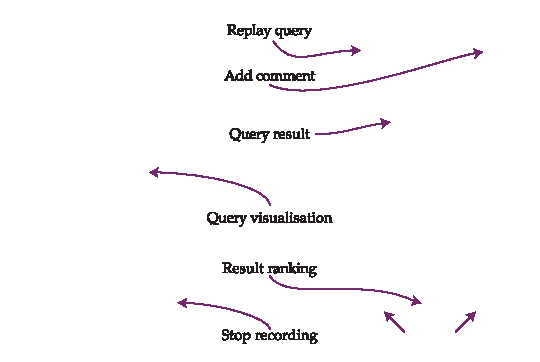
\includegraphics[width=\textwidth]{media/probe.pdf}}
\end{overpic}
    \caption{\textbf{Figure 1:} The media retrieval demonstrator app's screens for querying (left) and viewing/rating query results (right).\label{Fig-probe}\vspace{26em}}
\end{figure}


\makeatletter
\@openrightfalse
\makeatother

\tocchapter{Evaluation, Feedback and Refinement}

\makeatletter
\@openrighttrue
\makeatother


Having built an Information Retrieval (IR) system prototype, the next phase in this co-development pipeline is to showcase the system to the community with whom we are developing, therefore closing the feedback loop so essential to our developmental approach. 
To facilitate such evaluation and discussion, we suggest that the IR system is demonstrated and presented to community members via the Android app detailed in the previous section.


\section{In-person quantitative evaluation guidelines}
Recall that the goal of the spoken content retrieval system is to return the ``correct'' piece of content that is the closest match to the user's spoken query.
To assess our system's quality, then---and monitor how this quality increases or decreases after each new development/building/training iteration---we require some method of operationalising and scoring this.
Also useful to monitor is whether such system success/quality is uniform across all content items, or whether there are some types of ``content'' which give rise to more frequent false positive or false negative results. 

Here, then, we outline a quantitative evaluation study framework which can be used for this purpose.
Note that we present this evaluation methodology as an in-person study or workshop focusing on images as content items, but amendments could be made to focus on different types of content or to turn this into a remote task (through collaboration with community liaisons, using video-calling platforms, etc).

 
\section{Study setup}
To conduct this study (in-person), the following materials are required:
\begin{itemize}
    \item A phone with the media retrieval demonstrator app installed
    \item Paper printouts of all images in the IR system's database
\end{itemize}

The number of participants to be involved is up to the research team and community liaison but, if possible, the group should be representative of community demographics.
If this is not possible (for instance, if there ends up being a skew towards younger generations due to community members' availability), ensure to factor this into results analysis and interpretation.

Another factor that is important to consider during participant recruitment is whether community members have been involved in previous system development workshops, especially through any direct data-contribution.
One may want to set the constraint that only community members who have \textit{not} previously contributed data be included in such an evaluation study.
Alternatively, this study could be repeated with multiple groups: once with a group of community members who have been part of previous workshops/data-collection activities and thus better understand the system context; and once with a group who are less familiar. 

This study should be conducted somewhere in the community where there is likely to be minimal disturbance, for example inside a community member's home.
As the study will involve each participant taking it in turns to carry out a set of specific tasks, we recommend holding all participant sessions consecutively and on the same day to minimise participants consulting with one another about the tasks at hand.


\section{Evaluation tasks}
Once the setup above has been established, the following tasks can be conducted with each participant individually:

\textbf{Task 1: querying individual photos:} Keeping the full set of printed photos hidden from the participant, shuffle the photos to randomise their order.
Next, show the photos one at a time by holding them up for the participant to see.
Each time after showing a photo, ask the participant to use the media retrieval demonstrator app to record a query that they would expect to bring up this photo.
Once the app has returned a photo in answer to this query, rate this returned photo result using the buttons on the app's photo results screen (that is, confirm whether or not the app's returned photo matches that which was initially shown to the participant).
If the app's first response is incorrect, continue to cycle through the subsequent images that are returned, marking them as incorrect until the ``correct'' image is reached).
After an image has been shown, remove it from the photo set.
If any of the query recordings are interrupted (e.g., by background noise, another person entering the room, etc), this can be noted using the ``recording comments'' function on the corresponding image's results screen.
It is important to keep a note of these cases when it comes to analysing this task's results. 

\textbf{Task 2: querying the collection:} Spread out all of the printed photos on the floor; then point to an individual photo.
As with the first task, ask the participant to use the app to record a query that should bring up that photo as a result, and follow this by rating the returned photo results.
Point to another photo, and repeat the process until all photos have been covered.
The aim of this ``show the collection'' augmentation is to assess whether query framing---or indeed, query success---is affected when participants have contextual knowledge about the full corpus of images. 

For both tasks, the participant should be encouraged to speak naturally (rather than, for example, feeling obliged to take only a keyword-based approach) when interacting with the media retrieval app.


\section{Depicting and analysing results}
The data obtained from each of these tasks will take the following form.
Each image will have an associated set of queries (one for each participant who was shown that image during trials).
In turn, each of these queries will have an associated ``rank'' pertaining to where the ``correct' image was placed in the list of database images returned in response to the query.


\begin{figure}\centering
    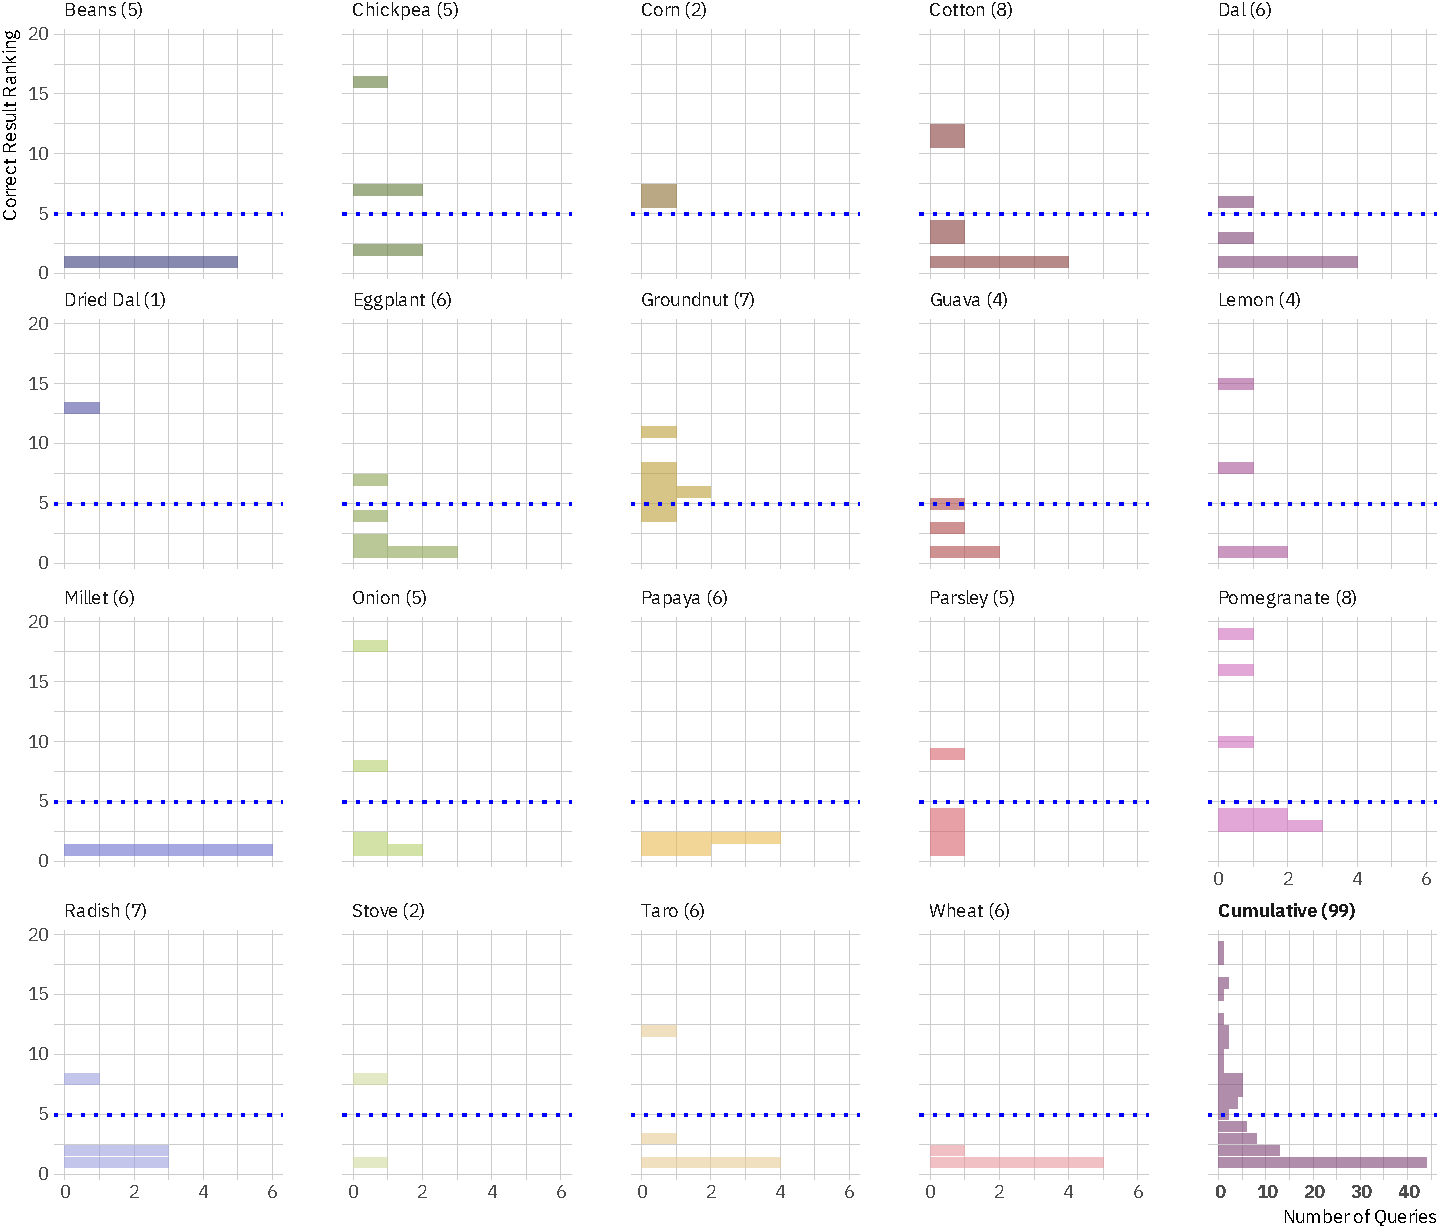
\includegraphics[width=\textwidth]{media/results}
    \caption{\textbf{Figure 2: }
    Distribution of result rankings for 99 spoken queries across 19 photos (pertaining to ``farming practices'') with top-5 results shown below the dotted blue line.}
    \caption{For example, the bar plot at the bottom left corner of the chart is captioned ``Radish (7)'' to indicate that the photo was of a radish plant and was shown to seven participants who each formulated their own query for that photo.
    This particular plot shows that across the seven queries the photo of the radish plant was returned as the 8\textsuperscript{th} ranked result once, the 2\textsuperscript{nd} ranked result three times and as the top result a further three times.
    A cumulative distribution combining results from all 19 photos is shown at the bottom right corner of the chart.
    \label{Fig-photo-rankings}\vspace{10em}}
\end{figure}

An example of how to visualise these distributions is shown on the following page.
We would recommend some form of data cleaning prior to this depiction and subsequent analysis; for example, we suggest excluding those queries that contained audio comment reminders that there had been an interruption during recording.

Whilst there are multiple ways in which this data could be analysed or summarised, some possible prompts include: 
\begin{itemize}
    \item Across all photos, what percentage of queries returned the correct image as a ``top-5'' result?
    \item Are there any commonalities between those queries that did not meet this threshold?
    For instance, do these queries focus on background elements of the image or aspects that are too closely related to topics demonstrated in other images?    
    \item Can any reasoning be identified to help with this analysis?\footnote{Note that analysis of query content should include community members and/or the community liaison, who will likely be able to add context to queries such as this.
}
\end{itemize}

Note also that both study tasks will give rise to such a data-set independently.
It is worth comparing and contrasting results across the two tasks to assess the role context plays in query design and success.


\section{Workshops to co-design, co-create and engage}
Moving on from quantitative evaluation, the media retrieval app's interactive demonstration capability can also be leveraged to engage and involve community members in more qualitative, discursive workshops surrounding system evaluation, improvement and future co-design.
In this section we provide some examples of workshops or discussion topics that could be used to spur useful and illuminating conversation around these areas.
As always, community demographics should be considered.
For example, involving community members from different generations is particularly important for this activity given topics pertaining to mobile phone usage and non-usage, fluency and literacy of varying languages, and so forth.

As a starting point, this phase of the language system development pipeline is a great chance to revisit with community members some of those questions or topics that were asked or explored in very early formative project phases.
It is possible that discussions surrounding day-to-day life and community and cultural norms evolve in very different ways, given the community's recent experiences, and new-found knowledge, of spoken language technology capabilities.
Particular topics that may be worth revisiting include:

\begin{itemize}
    \item \textbf{Current information seeking practices}: Starting a discussion surrounding this topic is a good way to begin to explore possibilities for future, more specific IR system use-cases.
    How do community members go about obtaining essential information in specific scenarios?
    For instance, this might involve the buying and selling of goods, seeking of health information, or the seeking of help and information to manage crop diseases and pests.
    Is the internet a useful resource in these scenarios?
    How is communication between involved parties conducted or facilitated?
    Is travel to neighbouring communities involved in order to obtain required information?
    Do community members rather get information in person than via a phone call or online resource, and why?
    \item \textbf{Language usage and practices}: It is also worth revisiting language norms, specifically relating to dissemination of information, or else engagement with technology.
    What are the community's language usage norms?
    Are multiple languages used?
    If so, are different languages constrained to different contexts or domains, or else used to obtain different types of information?
Are different languages perceived in different ways or associated with any connotations (which may need to be factored into future interaction designs)?
    \item \textbf{Multimedia usage and practices:} %
    Do community members regularly access multimedia content and, if so, where (e.g., sites such as YouTube)? What language(s) are to conduct these searches, and what language(s) is the multimedia available in?
    What interfaces are currently used to orchestrate searching (for example, voice search on smartphones, transliteration, etc)?
    Do community members create and share their own multimedia, or else want to/wish they had means to do so?
    If so, on what topics would this content be based?
    With whom might they want it to be shared (for example, family, friends, neighbouring communities, elders, younger generations)?   
\end{itemize}


\section{Community-generated media}
Another way to explore how such spoken IR technology could be extended is to assess what type of content community members themselves choose to generate and share with each other.
One way to orchestrate this without the privacy challenges of requesting existing private content is by hosting a workshop or activity in which participants are lent phones/devices (so that device preference or quality is not a factor), shown how to take photos and record video or audio, and then tasked to go out to record their own content. 

We recommend following these more open-ended or discursive activities by inviting back the same participants and asking, in light of recent discussions, how they may want or could imagine the spoken language technologies embodied and exemplified by the simple media retrieval app to be extended.

\begin{unmutehighlight}
\section*{Insights from a Banjara community}
When we conducted such an activity with a Banjara community, we found that people were particularly keen to record videos of themselves or others in the community carrying out day-to-day tasks such as cooking, weeding, or ploughing.

\vspace{1em}

Community members came up with a wide range of ideas for spoken Information Retrieval (IR) systems: 
\vspace{0.5em}
\begin{itemize}[leftmargin=*]
    \item Using the system to store and retrieve---and therefore share---songs 
    \item Documenting, and subsequently querying, how different communities carry out daily tasks pertaining to farming, cooking, buying and selling, and so on
\end{itemize}
\end{unmutehighlight}
\begin{unmutehighlight}
\begin{itemize}[leftmargin=*]
    \item Supporting the passing down, recording and disseminating of community traditions or knowledge (for example, methods in cooking or farming)
\end{itemize}
\end{unmutehighlight}


\tocchapter[Conclusion]{\texorpdfstring{\vspace{2.2em}}{}Concluding Remarks} %
At the start of this report we discussed the richness of speech as a form of human communication, and posed a challenge to others working in speech and language technology: to extend the benefits of speech-based interactive systems to more than just a small fraction of the world's languages.

Through the work outlined here we have been able to produce a blueprint for addressing this goal in a way that is responsible and inclusive, and also avoids the vast data harvesting associated with other state-of-the-art methods.
We have released our work as a set of open-source tools to support and inspire others wanting to work in this area. 

Our work continues, with further methodological and technological contributions planned.
We hope you will join us in this endeavour.



\includepdf[pages={1},offset=0 0mm,height=218mm]{media/cover-back}
\end{document}
